\section{正态近似误差}
\label{sec:clt-error}

中心极限定理是$n\to\infty$时的结论，它保证误差趋于零，却不告诉我们$n=100$时误差是$0.04$还是$0.4$。前面的例子已经给出一些具体数字：$\operatorname{Bin}(20,0.3)$在阈值$8$处差了$0.05$，十个指数等待时间的平均在均值处差了$0.042$。本节先确定比较的是哪一种误差，再在多一阶矩的条件下给出对所有阈值同时成立的上界。

\paragraph{比较什么}
设$F_n$是$Z_n$的分布函数。最常用的比较对象是两条分布函数之间的最大竖直距离
\begin{equation}
 D_n=\sup_{x\in\mathbb{R}}\bigl\lvert F_n(x)-\Phi(x)\bigr\rvert .
 \label{eq:clt-kolmogorov}
\end{equation}
它控制所有形如$\{Z_n\leq x\}$的事件，从而控制所有区间事件：$\mathbb{P}(a<Z_n\leq b)$与$\Phi(b)-\Phi(a)$之差不超过$2D_n$。由式~\eqref{eq:clt-iid-cdf}与$\Phi$的连续性，可以证明$D_n\to0$，但定理本身不给出速度。怎样利用这样的近似构造区间并评价其可靠性，属于统计推断的问题，可参考\BookChapterRef{chap:parametric-statistical-inference}{卷八第1章“参数化统计推断”}；这里只研究概率误差本身。

\subsection{Berry--Esseen界}
\label{sec:clt-berry-esseen}

定理~\ref{thm:clt-iid}的证明里，单个因子的误差用了二次界，因为只知道二阶矩。如果三阶绝对矩有限，就可以用三次界：每个因子的误差约为$\lvert t\rvert^3\mathbb{E}[\lvert Y\rvert^3]/(6n^{3/2})$，$n$个因子累计为$\lvert t\rvert^3\mathbb{E}[\lvert Y\rvert^3]/(6\sqrt{n})$。特征函数之差按$1/\sqrt{n}$缩小，分布函数之差也应当如此。

\begin{theorem}[Berry--Esseen界]
\label{thm:clt-berry-esseen}
设$X_1,X_2,\dots$独立同分布，方差$\sigma^2>0$，三阶绝对中心矩$\rho=\mathbb{E}[\lvert X_1-\mu\rvert^{3}]<\infty$。则存在与分布无关的常数$C$，使对每个$n\geq1$，
\begin{equation}
 \sup_{x\in\mathbb{R}}\bigl\lvert\mathbb{P}(Z_n\leq x)-\Phi(x)\bigr\rvert\leq\frac{C\rho}{\sigma^{3}\sqrt{n}} .
 \label{eq:clt-berry-esseen}
\end{equation}
\end{theorem}

这个上界称为\term{Berry--Esseen界}（Berry-Esseen bound）。目前已知可以取$C=0.4748$。证明的关键是一个光滑化不等式：把分布函数之差用特征函数之差在原点附近的积分来控制，再代入上面的三阶估计。这一不等式的推导与常数的优化都较长，读者可查阅~\scite{math-kallenberg2021probability}。

\paragraph{界的含义}
式~\eqref{eq:clt-berry-esseen}有三个特点。它对所有阈值$x$同时成立，所以是一致的；它控制的是概率之差，是绝对误差；它以$1/\sqrt{n}$的速度缩小，样本量变成四倍，误差界减半。分布的影响全部集中在比值$\rho/\sigma^3$上，这是标准化变量$Y$的三阶绝对矩$\mathbb{E}[\lvert Y\rvert^3]$。

这个比值至少是$1$。函数$u\mapsto u^{3/2}$在$[0,\infty)$上是凸函数，对非负变量$Y^2$用Jensen不等式，
\[
 \mathbb{E}\bigl[\lvert Y\rvert^{3}\bigr]=\mathbb{E}\bigl[(Y^2)^{3/2}\bigr]\geq\bigl(\mathbb{E}[Y^2]\bigr)^{3/2}=1 .
\]
等号对以等概率取$\pm1$的$Y$成立。比值越大，说明单项的取值越偏离“正负各一个标准差”，界越松。

\paragraph{三个分布的比值}
对$X\sim\operatorname{Bern}(p)$，$\lvert X-p\rvert$以概率$p$取$1-p$，以概率$1-p$取$p$，记$q=1-p$，
\[
 \rho=pq^3+qp^3=pq(p^2+q^2),\qquad \frac{\rho}{\sigma^3}=\frac{p^2+q^2}{\sqrt{pq}} .
\]
$p=1/2$时比值为$1$，$p=1/10$时为$0.82/0.3\approx2.733$。对$X\sim\operatorname{Exp}(1)$，$\sigma=1$，把积分在$x=1$处分开，
\[
 \int_1^{\infty}(x-1)^3\mathrm{e}^{-x}\,\mathrm{d}x=\frac{6}{\mathrm{e}},\qquad \int_0^1(1-x)^3\mathrm{e}^{-x}\,\mathrm{d}x=\frac{6}{\mathrm{e}}-2 ,
\]
前一个积分换元$u=x-1$后是$\mathrm{e}^{-1}\int_0^\infty u^3\mathrm{e}^{-u}\,\mathrm{d}u$，后一个由三次分部积分得到。合起来$\rho=12/\mathrm{e}-2\approx2.415$。

表~\ref{tab:clt-berry-esseen}比较$n=100$时的上界与精确的最大误差。最大误差由精确分布在所有跳点两侧逐一比较得到；指数情形用$\operatorname{Gamma}(n,1)$的分布函数在细网格上计算。

\begin{BookInlineTable}
 \centering
 \caption{$n=100$时Berry--Esseen上界（$C=0.4748$）与精确最大误差$D_{100}$的比较。}
 \label{tab:clt-berry-esseen}
 \begin{tabular}{lccc}
 \toprule
 单项分布 & $\rho/\sigma^3$ & 上界$C\rho/(\sigma^3\sqrt{100})$ & 精确$D_{100}$ \\
 \midrule
 $\operatorname{Bern}(1/2)$ & $1$ & $0.0475$ & $0.0398$ \\
 $\operatorname{Bern}(1/10)$ & $2.733$ & $0.130$ & $0.0832$ \\
 $\operatorname{Exp}(1)$ & $2.415$ & $0.115$ & $0.0133$ \\
 \bottomrule
 \end{tabular}
\end{BookInlineTable}

回到第~\ref{sec:clt-sample-mean}节掷$9604$次硬币的问题。比值为$1$，每个分布函数值的误差不超过$0.4748/\sqrt{9604}\approx0.0048$，区间概率是两个分布函数值之差，误差不超过$0.0097$。所以那里的“约为$0.95$”可以确切地写成“在$0.94$与$0.96$之间”。

表中硬币的上界只比实际误差大约五分之一，指数等待时间的上界却大了八倍多。图~\ref{fig:clt-berry-esseen-rate}在双对数坐标中画出$n$从$1$到$1000$的情形，所有误差曲线都以斜率$-1/2$下降，与上界平行，各自始终在自己的上界之下。

\begin{BookInlineFigure}
 \centering
 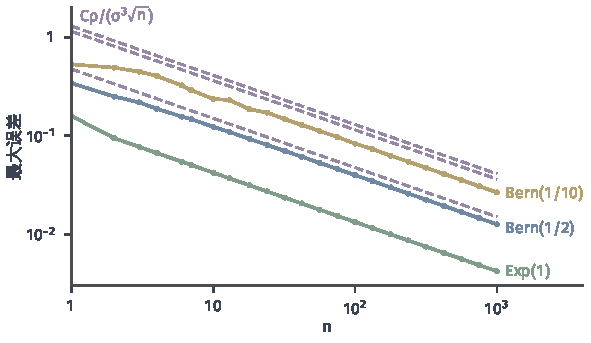
\includegraphics[width=100mm]{figures/07-probability/03-probability-limits/matplotlib/clt-berry-esseen-rate/figure.pdf}
 \caption{标准化和与$\mathcal{N}(0,1)$的精确最大误差$D_n$随$n$的变化，双对数坐标。蓝为$\operatorname{Bern}(1/2)$，黄为$\operatorname{Bern}(1/10)$，绿为$\operatorname{Exp}(1)$。紫色虚线是对应的Berry--Esseen上界$0.4748\rho/(\sigma^3\sqrt{n})$，自上而下依次属于$\operatorname{Bern}(1/10)$、$\operatorname{Exp}(1)$与$\operatorname{Bern}(1/2)$。}
 \label{fig:clt-berry-esseen-rate}
\end{BookInlineFigure}

\paragraph{速度不能更快}
$1/\sqrt{n}$的速度一般不能改进，硬币就是例子。$n$为偶数时，$Z_n$在$0$处有一个原子，质量是$\mathbb{P}(S_n=n/2)$，分布函数在那里跳起这么高，而$\Phi$是连续的。在跳点处，$F_n$的左极限与右值相差这个跳跃，它们与同一个数$\Phi(0)$的距离至少有一个不小于跳跃的一半。所以
\[
 D_n\geq\frac12\,\mathbb{P}\Bigl(S_n=\frac n2\Bigr)=\frac12\binom{n}{n/2}2^{-n} .
\]
$n=100$时右边是$\frac12\times0.0796=0.0398$，正好是表~\ref{tab:clt-berry-esseen}中的精确值。由Stirling公式，$\binom{n}{n/2}2^{-n}\approx\sqrt{2/(\pi n)}$，于是$D_n$至少约为$1/\sqrt{2\pi n}\approx0.399/\sqrt{n}$。这也说明常数$C$不能小于约$0.399$。

\paragraph{误差出现在哪里}
最大误差只是一个数，图~\ref{fig:clt-error-profile}画出带符号的误差$F_n(x)-\Phi(x)$随阈值的变化。指数等待时间的误差是一条光滑的波形，在中心附近为正、两侧为负，这是右偏造成的：均值处的分布函数值$0.542$超过$1/2$。硬币的误差是锯齿形，每过一个格点跳一次，幅度在中心最大；这一误差来自格点结构，任何光滑的近似都无法消除，连续性修正只是把阈值放到台阶中间以减小它。

\begin{BookInlineFigure}
 \centering
 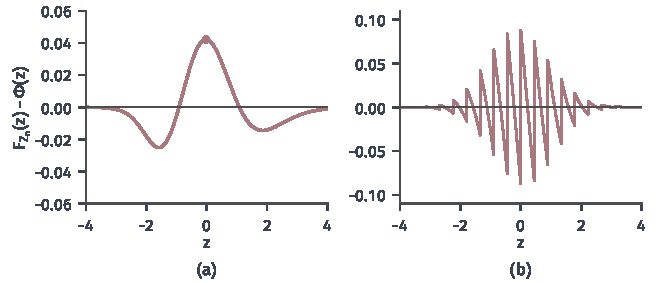
\includegraphics[width=112mm]{figures/07-probability/03-probability-limits/matplotlib/clt-error-profile/figure.pdf}
 \caption{带符号的误差$F_{Z_n}(z)-\Phi(z)$。(a)$\operatorname{Exp}(1)$，$n=10$，红点为最大误差$0.042$，位于$z\approx0$；(b)$\operatorname{Bern}(1/2)$，$n=20$，误差在每个格点处跳跃，最大约$0.088$。}
 \label{fig:clt-error-profile}
\end{BookInlineFigure}

\paragraph{非同分布的情形}
三角阵也有类似的界：若各项三阶绝对矩有限，$S_n/s_n$与$\mathcal{N}(0,1)$的分布函数最大距离不超过一个通用常数乘以
\[
 \frac{1}{s_n^3}\sum_{k=1}^{k_n}\mathbb{E}\bigl[\lvert X_{n,k}\rvert^{3}\bigr] ,
\]
这正是第~\ref{sec:clt-lyapunov}节$\delta=1$时的Lyapunov比值$\Lambda_n(1)$。Lyapunov条件因此不只保证收敛，在$\delta=1$时还直接给出了误差的量级。例A中$\Lambda_n(1)\approx27/(16\sqrt{n})$，误差也按$1/\sqrt{n}$缩小。

\subsection{近似的适用范围}
\label{sec:clt-applicability}

“正态近似可用”这句话要说清楚用于什么精度。表~\ref{tab:clt-accuracy}列出三种不同的要求。前两种已经讨论过；第三种在计算罕见事件的概率时常常遇到，Berry--Esseen界对它几乎没有帮助。

\begin{BookInlineTable}
 \centering
 \caption{正态近似的三种精度要求。}
 \label{tab:clt-accuracy}
 \begin{tabular}{lll}
 \toprule
 精度要求 & 含义 & 本章的依据 \\
 \midrule
 渐近收敛 & 误差随$n$趋于零 & 二阶矩或Lindeberg条件 \\
 一致绝对误差 & 给定$n$时的误差上界 & 三阶矩，Berry--Esseen界 \\
 尾概率相对误差 & 近似值与真值之比 & 本章没有给出 \\
 \bottomrule
 \end{tabular}
\end{BookInlineTable}

\paragraph{小尾概率}
设$p_n(z)=\mathbb{P}(Z_n\geq z)$。由式~\eqref{eq:clt-berry-esseen}，取左极限后同样有
\[
 \bigl\lvert p_n(z)-(1-\Phi(z))\bigr\rvert\leq\frac{C\rho}{\sigma^3\sqrt{n}} ,
\]
右边与$z$无关。当$z$较大时，$1-\Phi(z)$本身可能是$10^{-4}$甚至更小，而右边是$0.1$量级，这个界不能说明近似值有一位有效数字是对的。

十个指数等待时间的精确右尾与高斯近似是
\[
 \begin{aligned}
 z=2:&\quad 0.0369 &&\text{对}\quad 0.0228,\\
 z=3:&\quad 0.00672 &&\text{对}\quad 0.00135,\\
 z=4:&\quad 1.01\times10^{-3} &&\text{对}\quad 3.17\times10^{-5},\\
 z=5:&\quad 1.29\times10^{-4} &&\text{对}\quad 2.87\times10^{-7} .
 \end{aligned}
\]
比值依次约为$1.6$、$5.0$、$32$、$450$。绝对误差都不超过$0.015$，与Berry--Esseen界并不矛盾；相对误差却越来越大。左尾的情形更极端：$S_{10}>0$，所以$Z_{10}>-\sqrt{10}$，$\mathbb{P}(Z_{10}\leq-\sqrt{10})=0$，而高斯近似给出$\Phi(-\sqrt{10})\approx7.8\times10^{-4}$。

图~\ref{fig:clt-relative-tail}在对数纵轴上画出两侧的尾部。右偏的分布右尾比高斯厚，左尾比高斯薄而且在有限处截断。对数坐标暴露出来的这些差别，在普通坐标中都挤在零附近，看不出来。

\begin{BookInlineFigure}
 \centering
 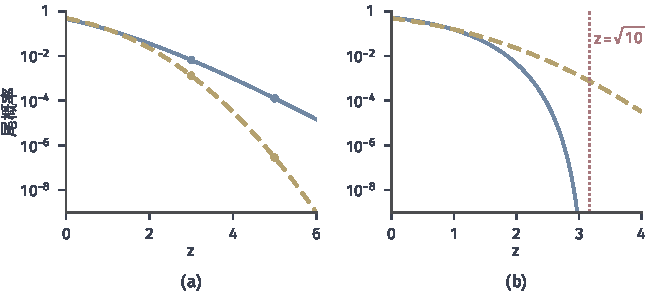
\includegraphics[width=112mm]{figures/07-probability/03-probability-limits/matplotlib/clt-relative-tail/figure.pdf}
 \caption{$n=10$个$\operatorname{Exp}(1)$之和标准化后的尾概率，纵轴为对数刻度。蓝线为精确值，黄色虚线为高斯近似。(a)右尾$\mathbb{P}(Z_{10}\geq z)$与$1-\Phi(z)$，圆点标出$z=3,5$；(b)左尾$\mathbb{P}(Z_{10}\leq-z)$与$\Phi(-z)$，精确左尾在$z=\sqrt{10}$（红色点线）处降为零。}
 \label{fig:clt-relative-tail}
\end{BookInlineFigure}

中心极限定理描述的是距中心几个标准差以内的“典型”波动；离中心越远，概率越依赖单项分布的尾部形状，而不仅是均值和方差。估计罕见事件的概率，应当直接计算精确分布，或使用第~\ref{chap:tail-probabilities}章基于指数矩的上界，它们的误差是按尾概率本身的大小来衡量的。

\paragraph{三阶矩无穷的情形}
Berry--Esseen界需要三阶绝对矩，中心极限定理只需要二阶矩，两者之间有一段空隙。取第~\ref{chap:tail-probabilities}章参数为$3$的Pareto分布，配上等概率的正负号，得到密度
\[
 f(x)=\frac32\lvert x\rvert^{-4},\qquad \lvert x\rvert\geq1 .
\]
它关于原点对称，均值为零。二阶矩与三阶绝对矩分别是
\[
 \mathbb{E}[X^2]=2\int_1^{\infty}x^2\cdot\frac32x^{-4}\,\mathrm{d}x=3,\qquad
 \mathbb{E}\bigl[\lvert X\rvert^3\bigr]=3\int_1^{\infty}x^{-1}\,\mathrm{d}x=\infty .
\]

方差有限，定理~\ref{thm:clt-iid}适用，$S_n/\sqrt{3n}\xrightarrow{\mathrm{d}}\mathcal{N}(0,1)$。图~\ref{fig:clt-pareto-third}的模拟也显示出钟形。可是$\rho=\infty$，式~\eqref{eq:clt-berry-esseen}的右边是无穷，不提供任何信息。收敛的速度需要另作分析：模拟中$\mathbb{P}(\lvert Z_n\rvert\leq0.5)$在$n=10$与$n=1000$时分别约为$0.402$与$0.392$，高斯值是$0.383$，$n=1000$时仍有约$0.009$的偏差，大于模拟本身约$0.003$的标准误差。

\begin{BookInlineFigure}
 \centering
 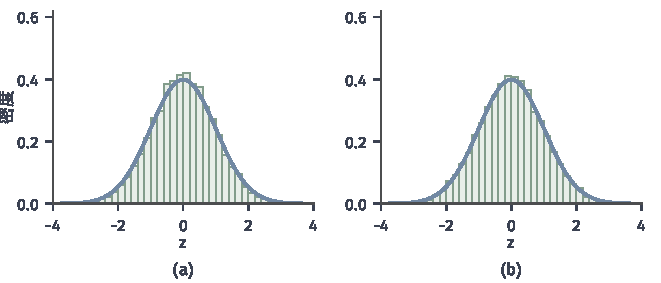
\includegraphics[width=112mm]{figures/07-probability/03-probability-limits/matplotlib/clt-pareto-third/figure.pdf}
 \caption{对称Pareto单项（密度$\frac32\lvert x\rvert^{-4}$，$\lvert x\rvert\geq1$，方差$3$，三阶绝对矩无穷）的标准化和$S_n/\sqrt{3n}$的直方图（浅绿，$20000$次重复，种子$11$）与$\varphi$（蓝）。(a)$n=10$；(b)$n=1000$。}
 \label{fig:clt-pareto-third}
\end{BookInlineFigure}

这个例子与第~\ref{sec:clt-lyapunov}节的比较是同一回事：收敛只看二阶矩，速度要看更高阶的矩。说“$n$足够大时可以用正态近似”之前，应当先问单项分布有没有有限的三阶矩，比值$\rho/\sigma^3$有多大，以及要计算的是典型区间的概率还是罕见事件的概率。
